\documentclass[12pt]{beamer}

\usepackage{cmap}
\usepackage[T2A]{fontenc}
\usepackage[utf8]{inputenc}
\usepackage[russian]{babel}
\usepackage{graphicx}
\usepackage{amsthm,amsmath,amssymb}
\usepackage{enumerate}
\usepackage{datetime}
\usepackage{minted}
\usepackage{fancyhdr}
\usepackage{lastpage}
\usepackage{color}
\usepackage{verbatim}
\usepackage{tikz}
\usepackage{euler}
\usepackage{eulervm}
\usepackage{dsfont}
\usepackage{beamerthemesplit}

\setcounter{page}{1}
\pagestyle{empty}

\mode<presentation>{}
\usetheme{Warsaw}
\usecolortheme{beaver}

\title[kittens] {Laser Kittens}
\author[Maxim Surkov, Konstantin Makhnev]
{Maxim Surkov \and Konstantin Makhnev}
\institute[Abstract University]
{
  Higher School of Economics
}
\date[date]
{April 3, 2019}
\subject{Computer Science}

\setbeamertemplate{footline}[frame number]

\AtBeginSection[]
{
  \begin{frame}
    \frametitle{Table of Contents}
    \tableofcontents[currentsection]
  \end{frame}
}
\addtobeamertemplate{navigation symbols}{}{%
    \usebeamerfont{footline}%
    \usebeamercolor[fg]{footline}%
    \hspace{1em}%
    \insertframenumber/\inserttotalframenumber
}



\begin{document}

\frame{\titlepage}

\section[Section] {Описание проекта}

\begin{frame}
    \frametitle{Описание проекта}
    \begin{columns}[T]
     \begin{column}[T]{\textwidth / 2}
        Игра на основе {\bf лазеров} и {\bf объектов} с ними взаимодействующих
     \end{column}
     \begin{column}[T]{\textwidth / 2}
         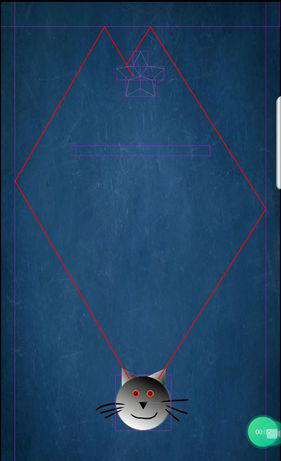
\includegraphics[width = 3cm]{cutmypic.png}
     \end{column}
     \end{columns}
\end{frame}

\begin{frame}
    \frametitle{Что уже сделано}
    \begin{enumerate}
        \item Меню и найстройки
        \item Выбор уровня
        \item Управление игроком
        \item Лазеры, зеркала, звёзды
        \item Демо-уровень
        \item Звуковые эффекты
    \end{enumerate}
\end{frame}

\begin{frame}
    \frametitle{Идеи}
    \begin{enumerate}
        \item Большая карта
        \item Несколько котиков
        \item Управление с помощью акселерометра
        \item Двери и ключи
        \item Преломление
        \item Terra Incognita
    \end{enumerate}
\end{frame}

\begin{frame}
    \frametitle{Что хотим добавить}
    \begin{enumerate}
        \item Google account
        \item Статистика (базы данных)
        \item Дизайн, анимация (картинки котиков!)
    \end{enumerate}
\end{frame}

\section[Section] {Демонстрация}

\end{document}
